Definition of the process. \\
Explaining the various contributions. \\
Show few Feynman diagrams and explain that it possesses also tri-boson contributions in the s-channel. \\
This is explained in some details in Ref.~\cite{Biedermann:2017bss}.

\begin{figure}[t]
\begin{center}
          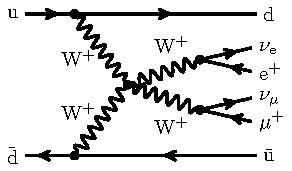
\includegraphics[width=0.30\linewidth]{feynman/LO_EW_5}
          \raisebox{.5ex}{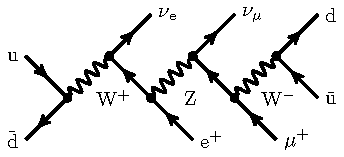
\includegraphics[width=0.35\linewidth]{feynman/LO_EW_2}}
          \raisebox{-1.8ex}{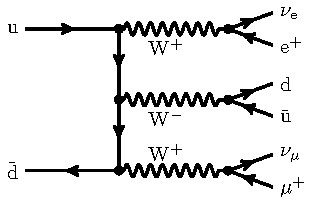
\includegraphics[width=0.32\linewidth]{feynman/LO_EW_3}}
\end{center}
        \caption{Sample tree-level diagrams that contribute to the process $\Pp\Pp\to\mu^+\nu_\mu\Pe^+\nu_{\Pe}\Pj\Pj$ at order $\mathcal{O}{\left(\alpha^{6}\right)}$.
        In addition to typical VBS contribution (left), this order also possesses $s$-channel (middle) and tri-boson contributions (right). }
\label{diag:LO}
\end{figure}
